\section{Evaluation}
\label{sec:evaluation}

Cudele lets \oldcomment{users}\newcomment{administrators} construct
consistency/durability guarantees using well-established research techniques
from other systems; so instead of evaluating the scalability and performance of
the techniques themselves against other file systems, we show that (1) the
mechanisms we propose are useful for constructing semantics used by real
systems and (2) the techniques can work side-by-side in the same namespace for
common use cases\oldcomment{, and (3) the combination of these techniques can
help the system scale further when subtrees are coupled to the correct type of
application}.
%\newcomment{These techniques have already proven to be effective and scalable
%in systems that specialize an entire namespace according to a single
%optimization strategy ({\it e.g.}, Lustre, BatchFS, DeltaFS).} , so our
%evaluation explores the behavior of the consistency/durability mechanisms and
%their effect with and without isolation.}

\newcomment{\indent We graph standard deviations for three runs (sometimes
error bars are too small to see) and normalize results to make our results more
generally applicable to different hardware. We use a CloudLab cluster of 34
nodes connected with 10Gbit ethernet, each with 16 2.4 GHz CPUs, 128GB RAM, and
400GB SSDs.  Each node uses Ubuntu 14.04 and we develop on Ceph's Jewel
release, version 10.2.1, which was released in May 2016. We use 1 monitor
daemon, 3 object storage daemons, 1 metadata server daemon, and up to 20
clients.}  We scope the evaluation to one metadata server and scale the number
of parallel clients \newcomment{each doing 100K operations because 100K is the
maximum recommended size of a directory in CephFS. We scale to 20 clients
because, as shown in Section~\S\ref{sec:posix-overheads}, 20 clients is enough
to saturate the resources of a single metadata server.} This type of analysis
shows the capacity and performance of a metadata server with superior metadata
protocols, which should be used to inform \oldcomment{load
balancing}\newcomment{metadata distribution} across a \oldcomment{metadata}
cluster. Load balancing across a cluster of metadata servers with partitioning
and replication can be explored with something like
Mantle~\cite{sevilla:sc15-mantle}.  \newcomment{To make our results
reproducible, this paper adheres to The Popper
Convention~\cite{jimenez_popper_2016} so experiments can be examined in more
detail, or even re-run, by visiting the \texttt{[source]} link next to each
figure.  The source code for Cudele is available on a branch~\cite{docs:cudele}
of our Ceph fork.}

%\newcomment{\indent We understand concerns about cluster size and network, especially
%for systems aimed at HPC but our evaluation focuses on verifying the behavior
%of different techniques in the same global namespace. 


%\begin{table}
%\begin{tabular}{ r | l | l}
%  Cluster  & Hardware               & Software \\\hline
%  In-House & 15 nodes, 4 2GHz CPUs  & Ubuntu 12.04, 1 MON\\
%           & 8GB RAM, SSD           & 1 MDS, 8 OSDs, 8 Clients\\
%  CloudLab & 34 nodes, 16 2.4GHz CPUs & Ubuntu 14.04, 1 MON\\
%           & 128GB RAM, SSD         & 1 MDS, 3 OSDs, 29 Clients
%\end{tabular}
%\caption{In-House used for microbenchmarks, CloudLab for Use Cases. MON is
%monitor daemon, MDS is metadata server daemon, and OSDs are object storage
%daemons.\label{table:clusters}} 
%\end{table}

\subsection{Microbenchmarks}
\label{sec:microbenchmarks}
\begin{figure}[tb]
\centering
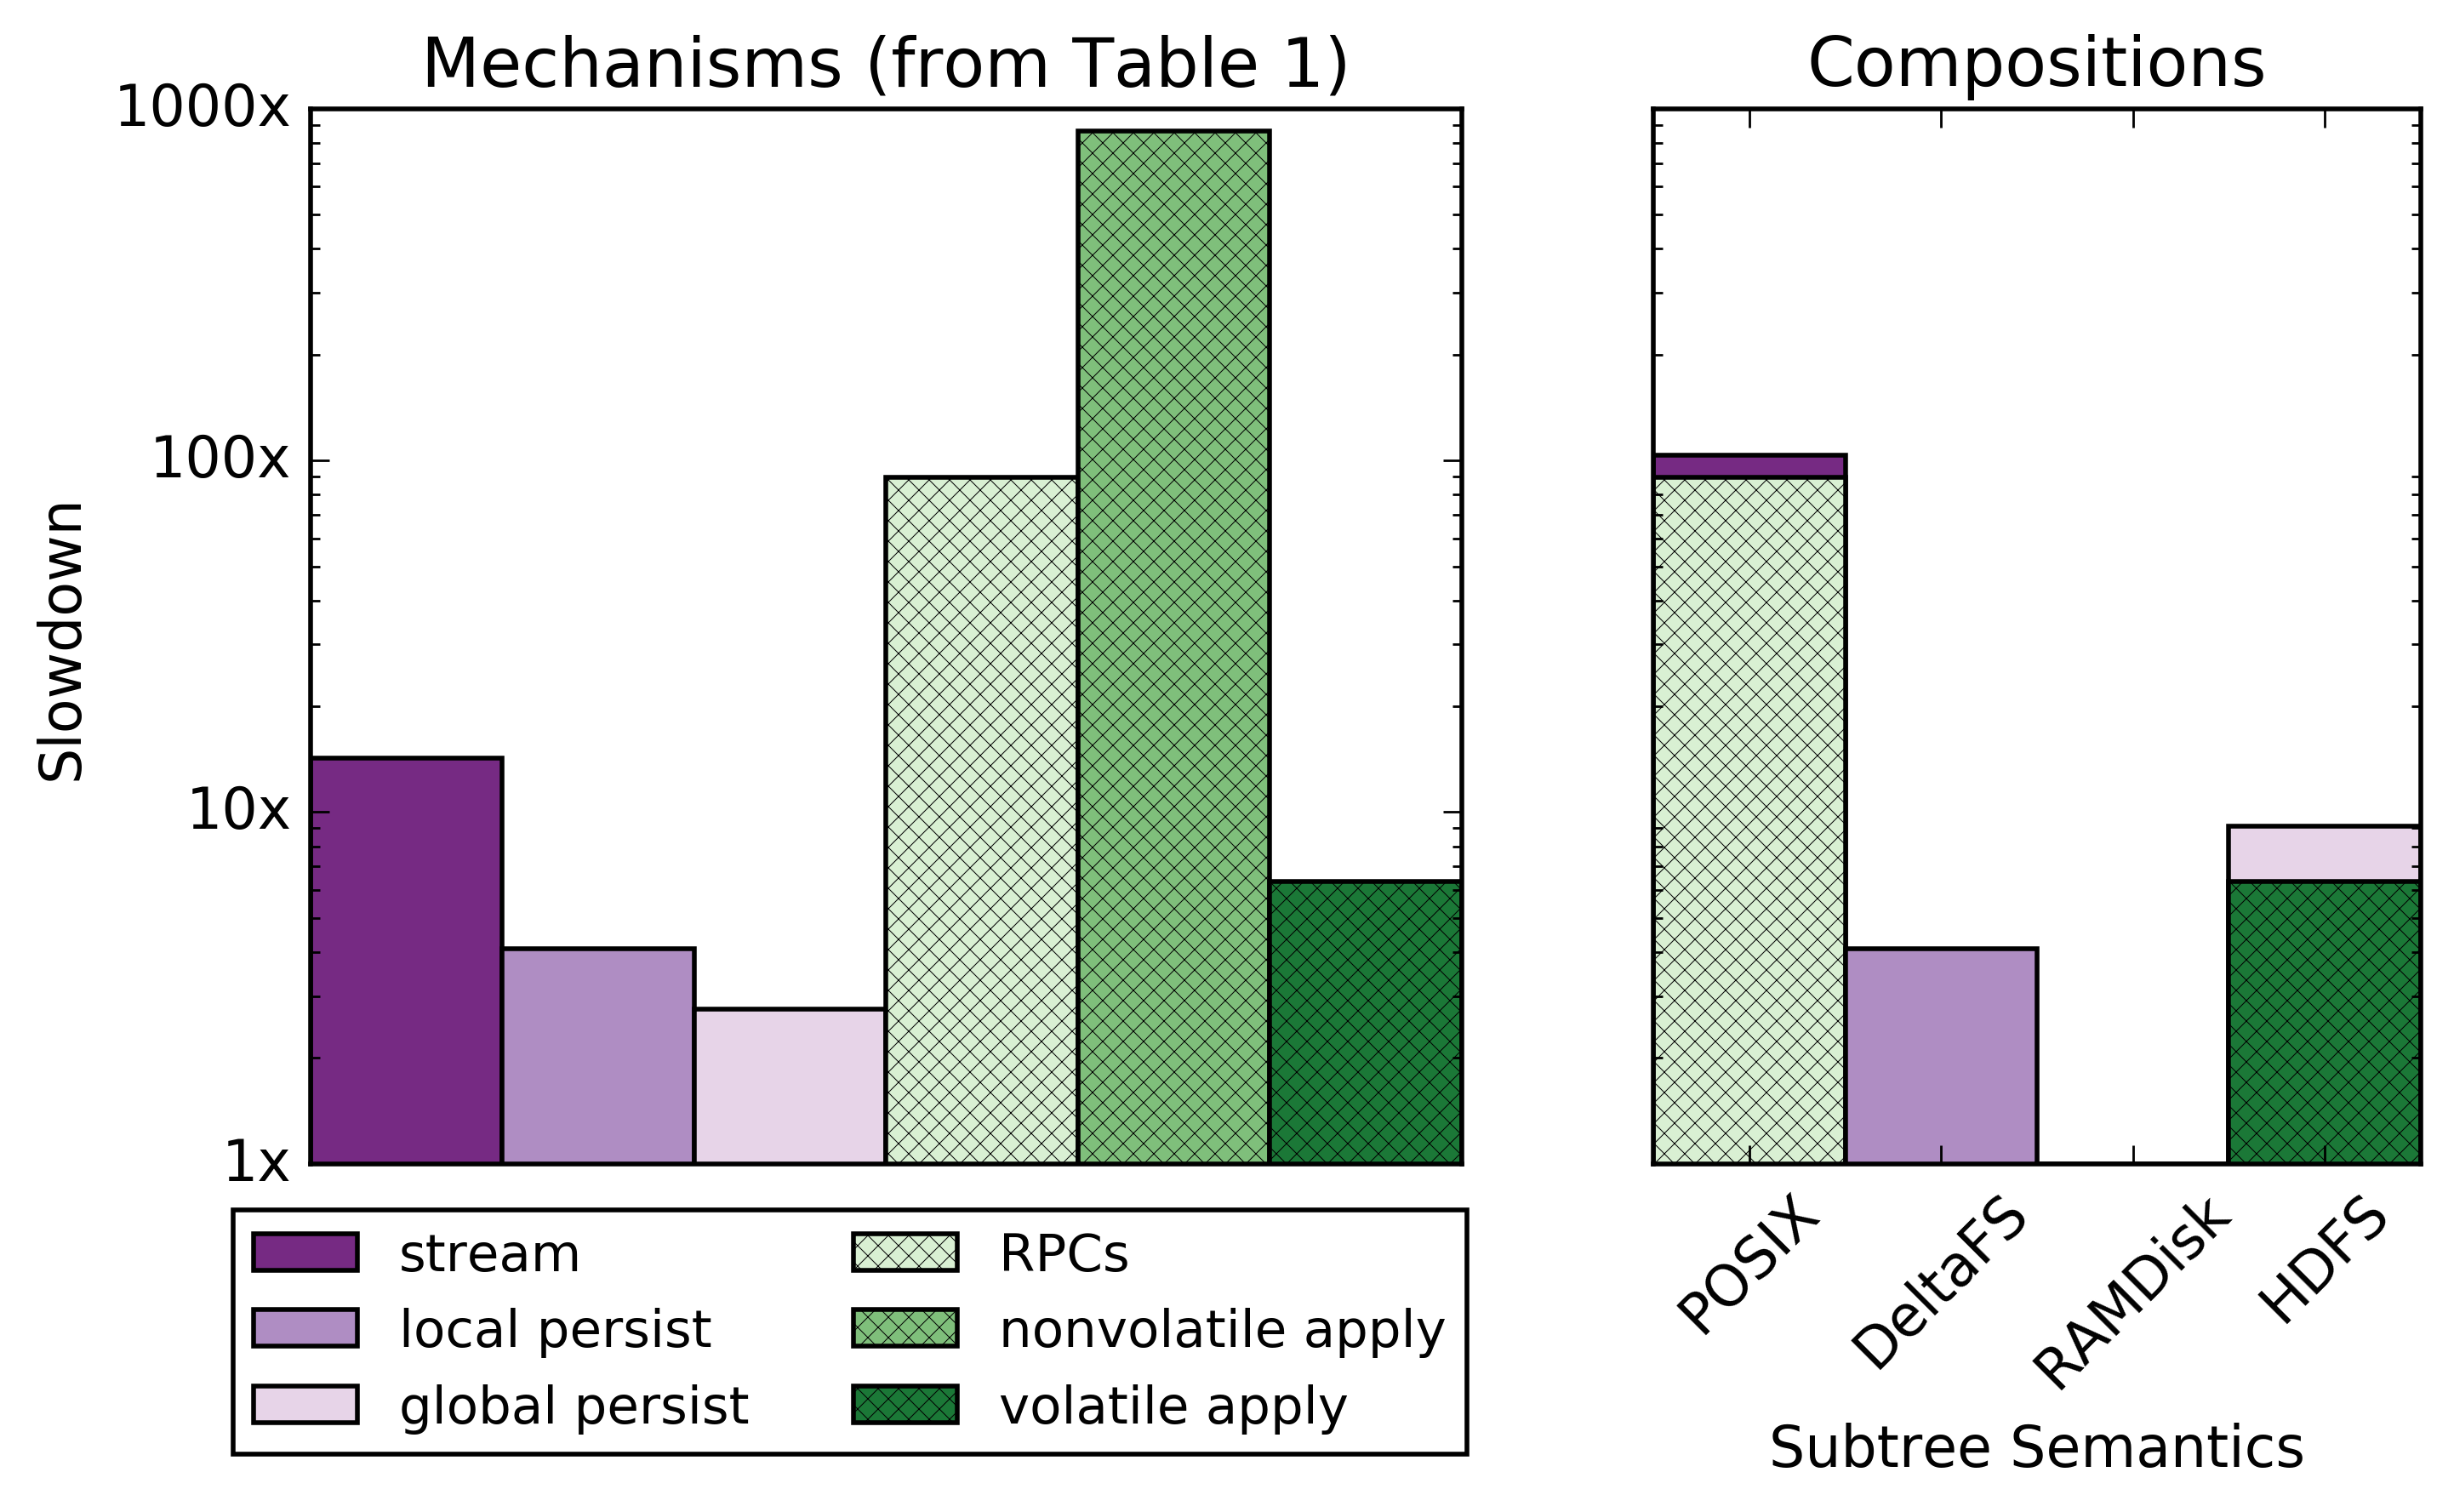
\includegraphics[width=0.5\linewidth]{./chapters/cudele/figures/composable-mechanisms.png}
\caption{
[\href{https://github.com/michaelsevilla/cudele-popper/blob/master/experiments/cudele-mechanisms/visualize/viz.ipynb}{source}]
\newcomment{Overhead of processing 100K create events for each mechanism in
\oldcomment{Table~\ref{table:mechanisms}}\newcomment{Figure~\ref{fig:decouple}},
normalized to the runtime of writing events to client memory. The far right
graph shows the overhead of building semantics of real world systems.}
\oldcomment{Performance of each mechanism (left) and building the
consistency/durability semantics of real-world systems (right) for 100K files
creates from a single client. Results are normalized to the runtime of writing
events to the client's in-memory journal.}\label{fig:composable-mechanisms}}
\end{figure}

%\begin{figure}[tb]
%\centering
%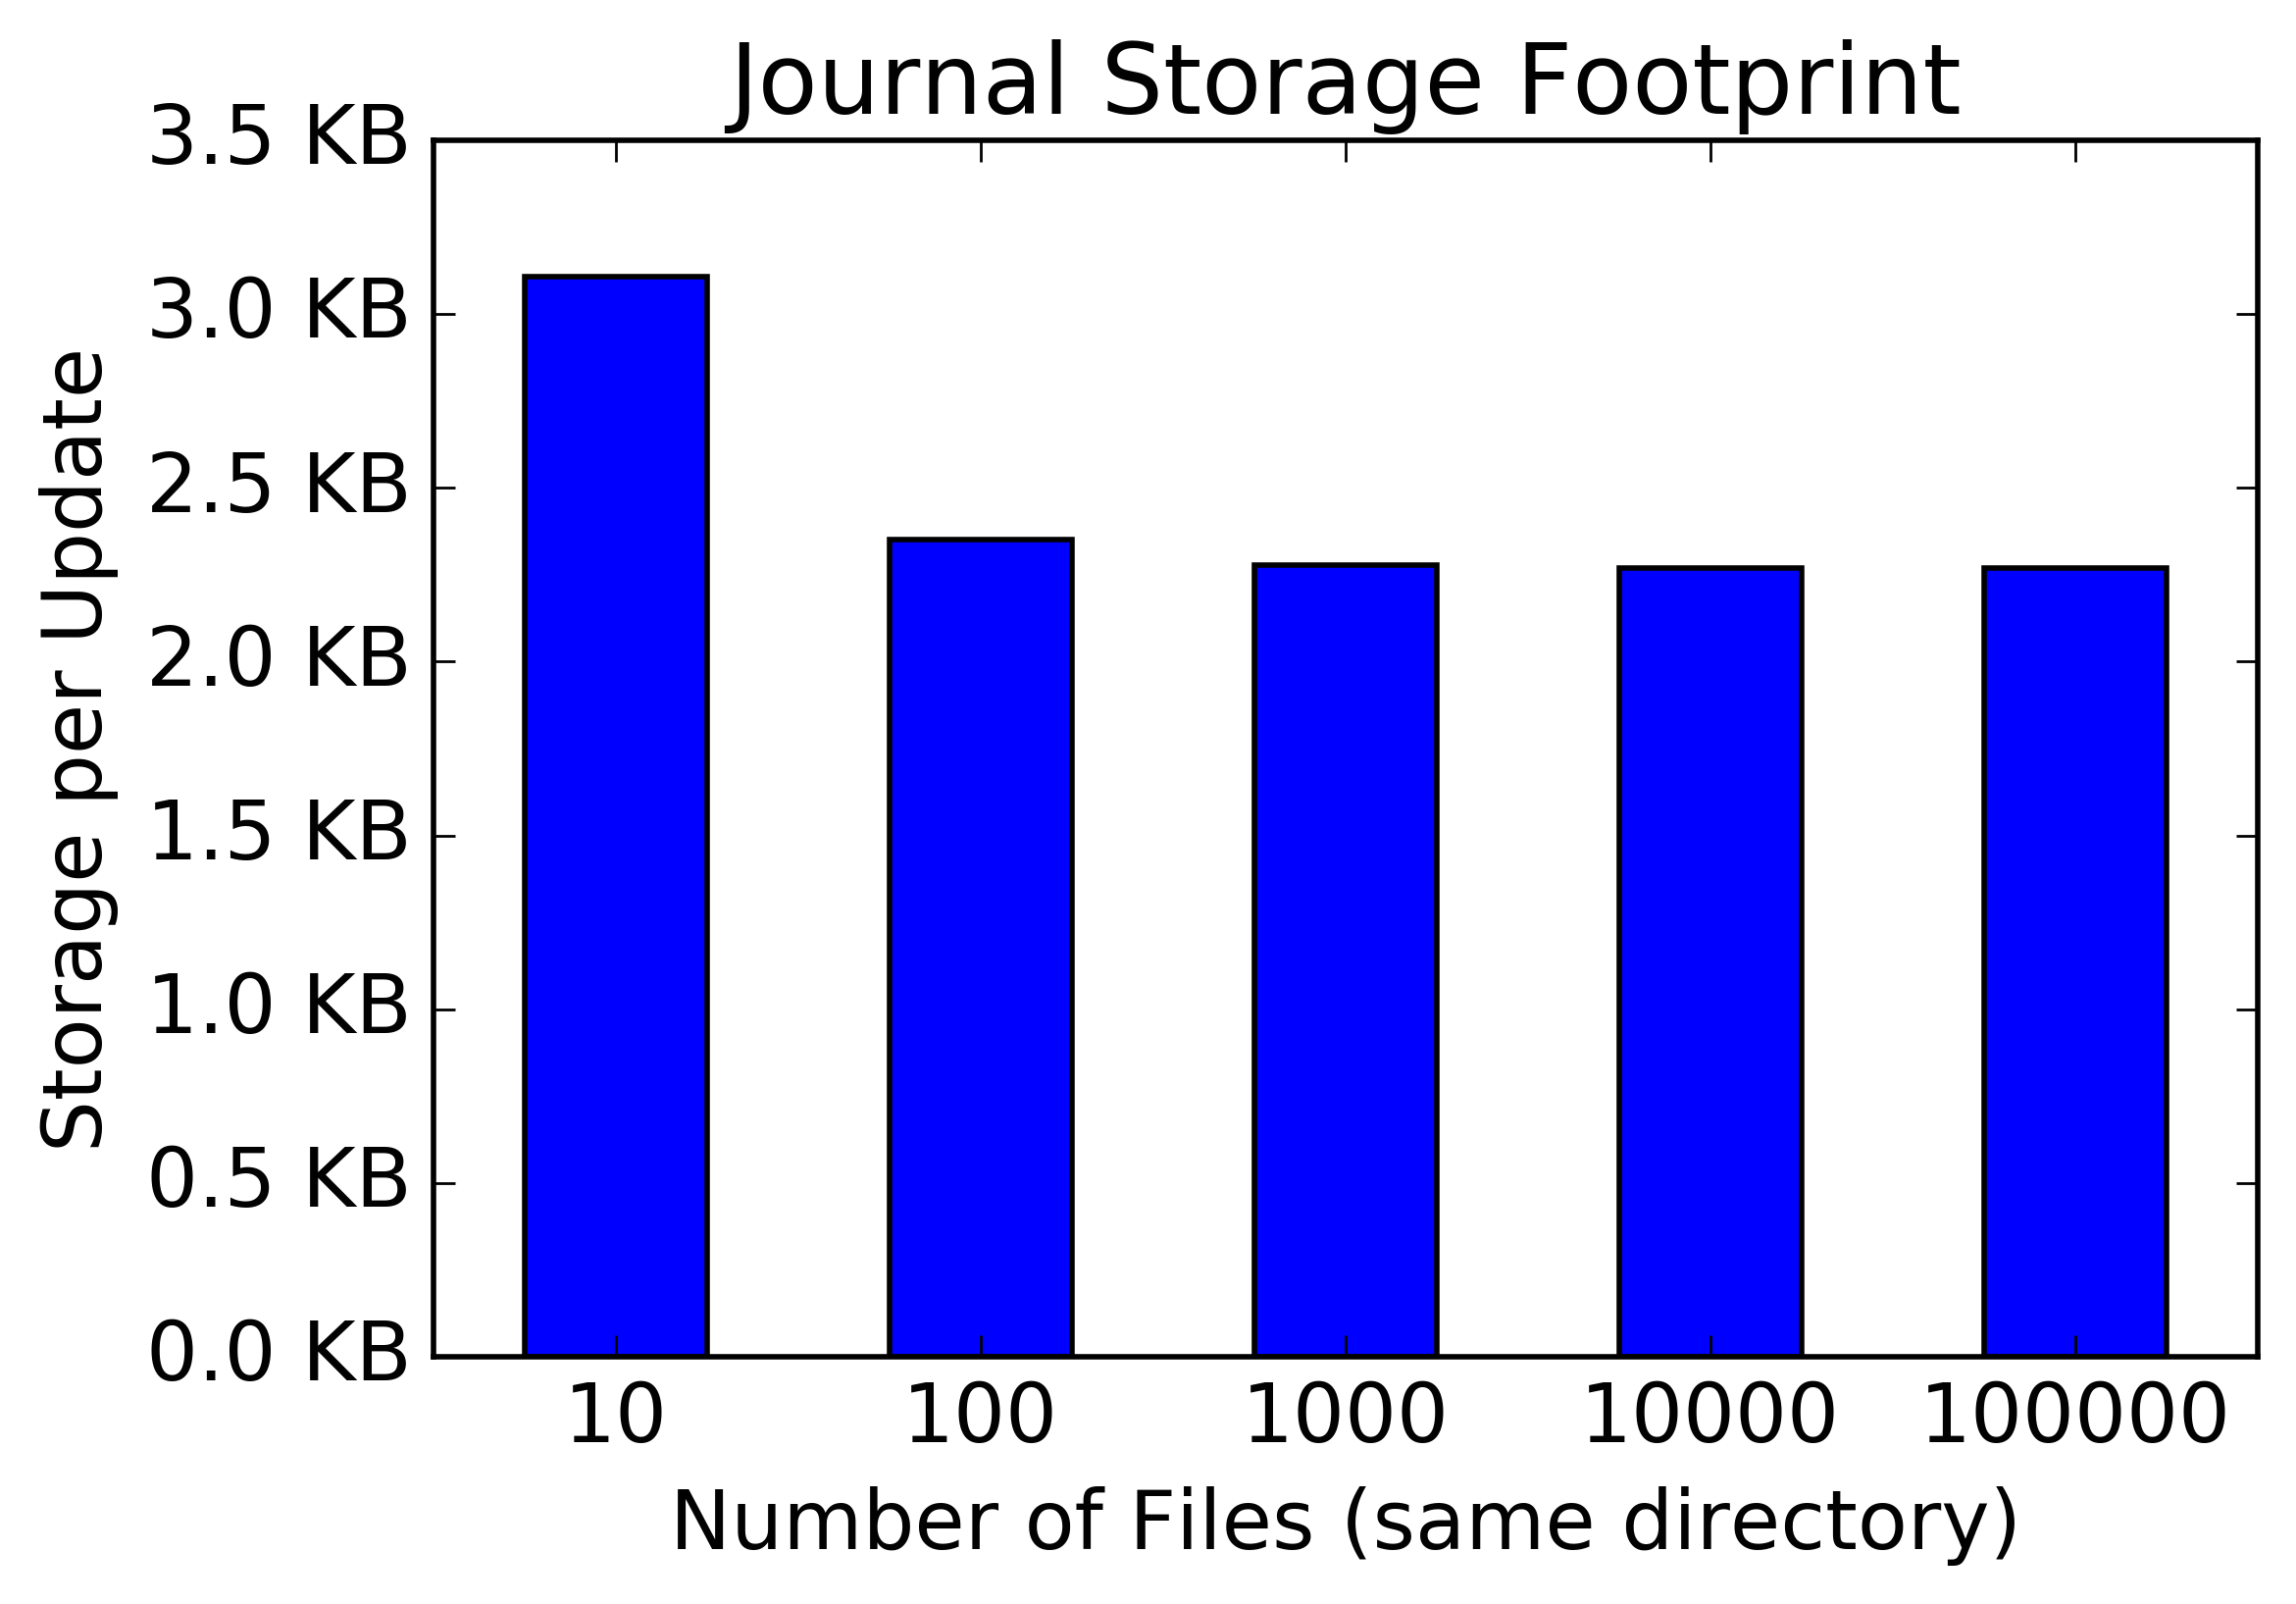
\includegraphics[width=1.0\linewidth]{./chapters/cudele/figures/behavior-journal-size.png}
%\caption{ [\href{https://...}{source}] Microbenchmark: storage footprint on
%client. The size of the client's journal scales with the number of
%updates.\label{fig:behavior-journal-size}}
%\end{figure}

\oldcomment{Figure~\ref{fig:composable-mechanisms} shows the runtime of the
Cudele mechanisms for a single client creating files in the same directory, }
\newcomment{We measure the overhead of each Cudele mechanism by having 1 client create
100K files in a directory for various subtree configurations.
Figure~\ref{fig:composable-mechanisms} shows the time that it takes each Cudele
mechanism to process all metadata events.  Results are} normalized to the time
it takes to write \oldcomment{100K file create}updates to the client's in-memory journal
({\it i.e.} the Append Client Journal mechanism), which is about 11K creates/sec.  \newcomment{The first graph
groups the consistency mechanisms, the second groups the durability mechanisms,
and the third has compositions representing real-world systems.} \oldcomment{Stream is an
approximation of the overhead and is calculated by subtracting the runtime of
the job with the journal turned off from the runtime with the journal turned
on.  100K is the maximum recommended size of a directory in CephFS;
preliminary experiments with larger directory sizes show memory problems.}

{\it Poorly Scaling Data Structures:} Despite doing the same amount of work,
mechanisms that rely on poorly scaling data structures have large
slowdowns\oldcomment{ for the larger number of creates}. For example, RPCs has
a \oldcomment{\(90\times\)}\newcomment{\(17.9\times\)} slowdown because this
technique relies on internal directory data structures\newcomment{, which is a
well-known problem~\cite{ren:sc2014-indexfs}}. \oldcomment{It is a well-known
problem that directory data structures do not scale when creating files in the
same directory~\cite{ren:sc2014-indexfs} and any mechanism that uses these data
structures will experience similar slowdowns.} Other mechanisms that write
events to a journal experience a much less drastic slowdown because the journal
data structure does not need to be scanned for every operation.  Events are
written to the end of the journal without even checking the validity ({\it
e.g.}, if the file already exists for a create), which is another form of
relaxed consistency because the file system assumes the application has
resolved conflicting updates in a different way.

% RPCs vs. apply: calls to metadata server vs. RADOS TODO: why is apply so
% slow.  apply: no CephFS changes, pulls/pushes same RADOS obj.  v_apply vs.
% apply/persist: communicating through RADOS
{\it Overhead of \oldcomment{RPCs}\newcomment{Consistency}:} RPCs is
\oldcomment{\(66\times\)}\newcomment{\(19.9\times\)} slower than Volatile Apply
because sending individual metadata updates over the network is costly.  While
RPCs sends a request for every file create, Volatile Apply \oldcomment{writes
all the updates to the in-memory journal and applies them}\newcomment{writes
directly} to the in-memory data structures in the metadata server. While
communicating the decoupled namespace directly to the metadata server
\newcomment{with Volatile Apply} is faster, communicating through the object
store \newcomment{with Nonvolatile Apply} is
\oldcomment{\(10\times\)}\newcomment{\(78\times\)} slower.  \oldcomment{{\it
Overhead of Nonvolatile Apply:} The cost of Nonvolatile Apply is much larger
than all the other mechanisms.  That mechanism}\newcomment{Nonvolatile Apply}
was not implemented as part of Cudele -- it was a debugging and recovery tool
packaged with CephFS. It works by iterating over the updates in the journal and
pulling all objects that {\it may} be affected by the update.  This means that
two objects are repeatedly pulled, updated, and pushed: the object that houses
the experiment directory and the object that contains the root directory ({\it
i.e.} \texttt{/}).  \oldcomment{The cost of communicating through the object
store is shown by comparing the runtime of Volatile Apply + Global Persist to
Nonvolatile Apply.  These two operations} \newcomment{Nonvolatile Apply
(\(78\times\)) and composing Volatile Apply + Global Persist (\(1.3\times\))}
end up with the same final metadata state but using Nonvolatile Apply is
clearly inferior.

% persist vs. save: one disk vs. many
{\it Parallelism of the Object Store:}
\newcomment{Stream, which is an approximation (journal on minus journal off), has
the highest slowdown at \(2.4\times\) because the overhead of maintaining and
streaming the journal is incurred by the metadata server}.  Comparing Local and
Global Persist demonstrates the bandwidth advantages of storing the journal in
a distributed object store. The Global Persist performance is \newcomment{only
\(0.2\times\) slower than Local Persist because Global
Persist}\oldcomment{\(1.5\times\) faster because the object store} is
leveraging the collective bandwidth of the disks in the cluster. This benefit
comes from the object store itself but should be acknowledged when making
decisions for the application; the bandwidth of the object store can help
mitigate the overheads of globally persisting metadata updates. The storage per
journal update is about 2.5KB. So the storage footprint scales linearly with
the number of metadata creates and suggests that updates for a million updates
in a single journal would be \newcomment{2.38GB}\oldcomment{2.5KB \(*\) 1
million files \(=\) 2.38GB.  Transfer times for payloads of this size in most
HPC/data center networks are reasonable.}

\oldcomment{\textbf{Takeaway}: measuring the mechanisms individually shows that their
overheads and costs can differ {\it by orders of magnitude}. We also show that
some mechanisms, like Nonvolatile Apply, are not worthwhile as currently
implemented.}

\begin{figure}[tb]
  \centering
  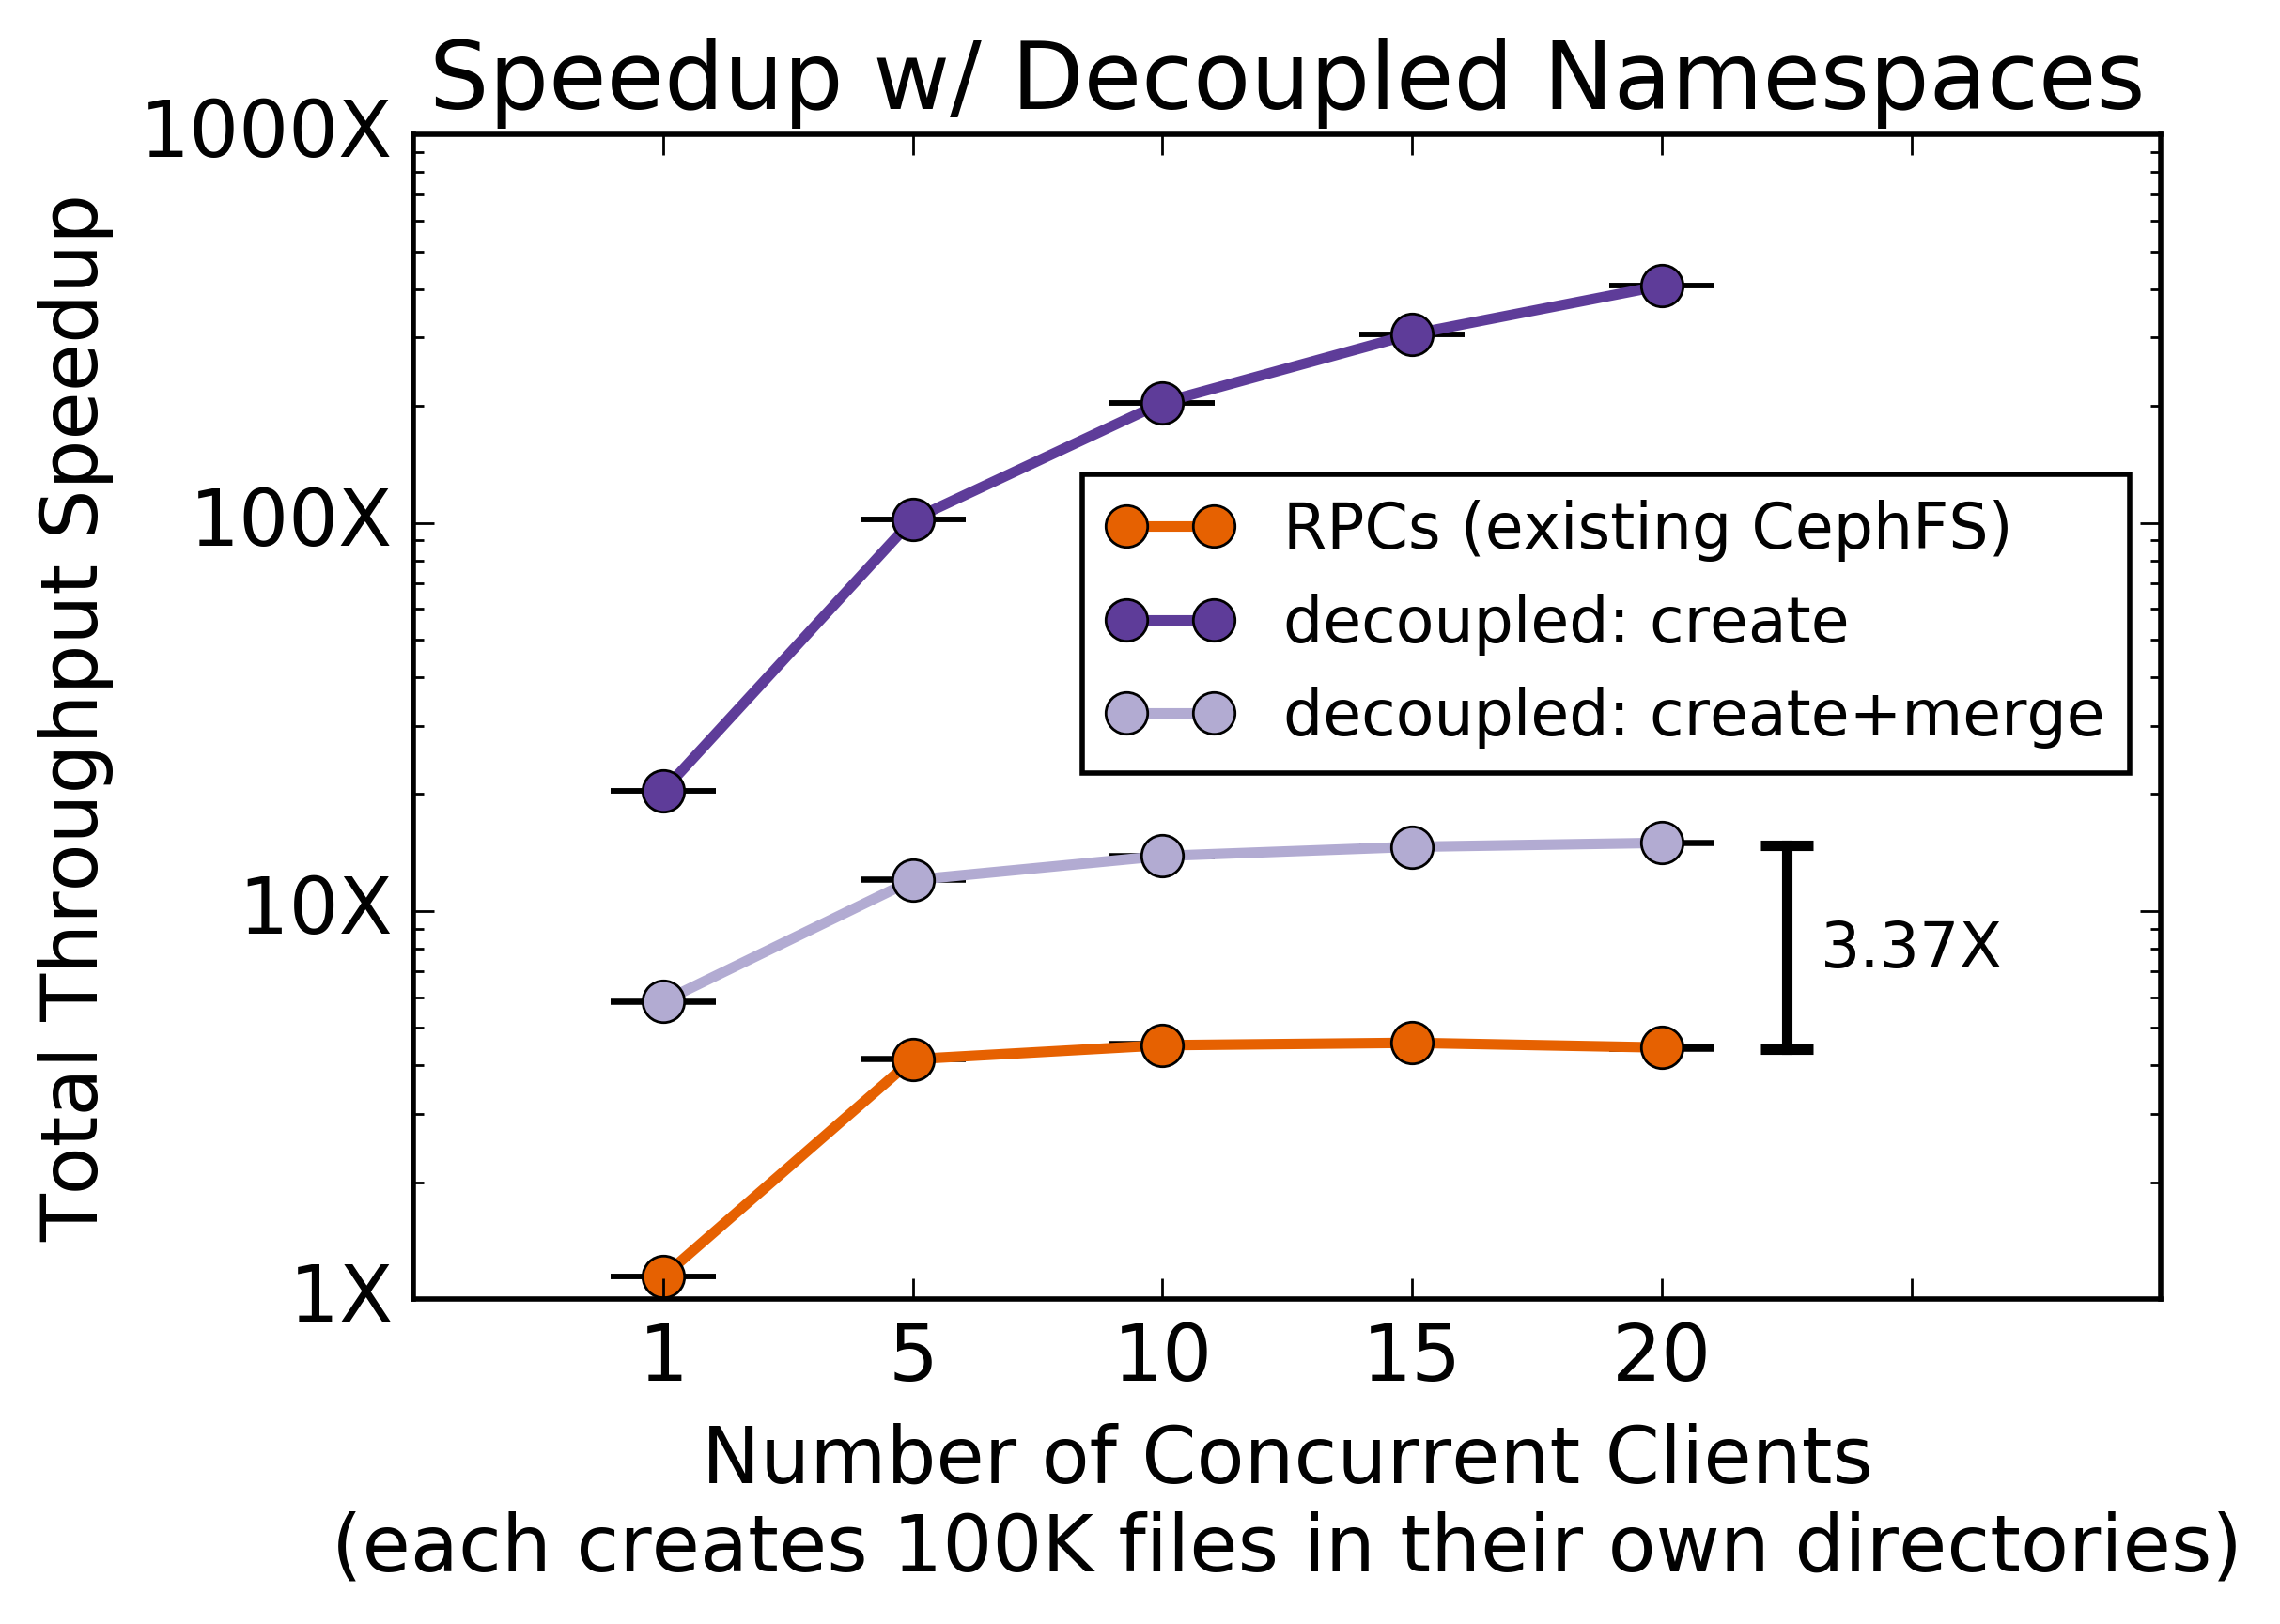
\includegraphics[width=0.5\linewidth]{./chapters/cudele/figures/mergescale.png}
  \caption{
  [\href{https://github.com/michaelsevilla/cudele-popper/blob/master/experiments/cudele-mergescale/visualize/viz.ipynb}{source}]
  The speedup of decoupled namespaces over RPCs for parallel creates on clients ;
  \texttt{create} is the throughput of clients creating files in-parallel and
  writing updates locally; \texttt{create+merge} includes the time to merge
  updates at the metadata server.  Decoupled namespaces scale better than RPCs
  because there are less messages and consistency/durability code paths are
  bypassed.}
  \label{fig:mergescale}
\end{figure}

\begin{figure}[tb]
  \centering
  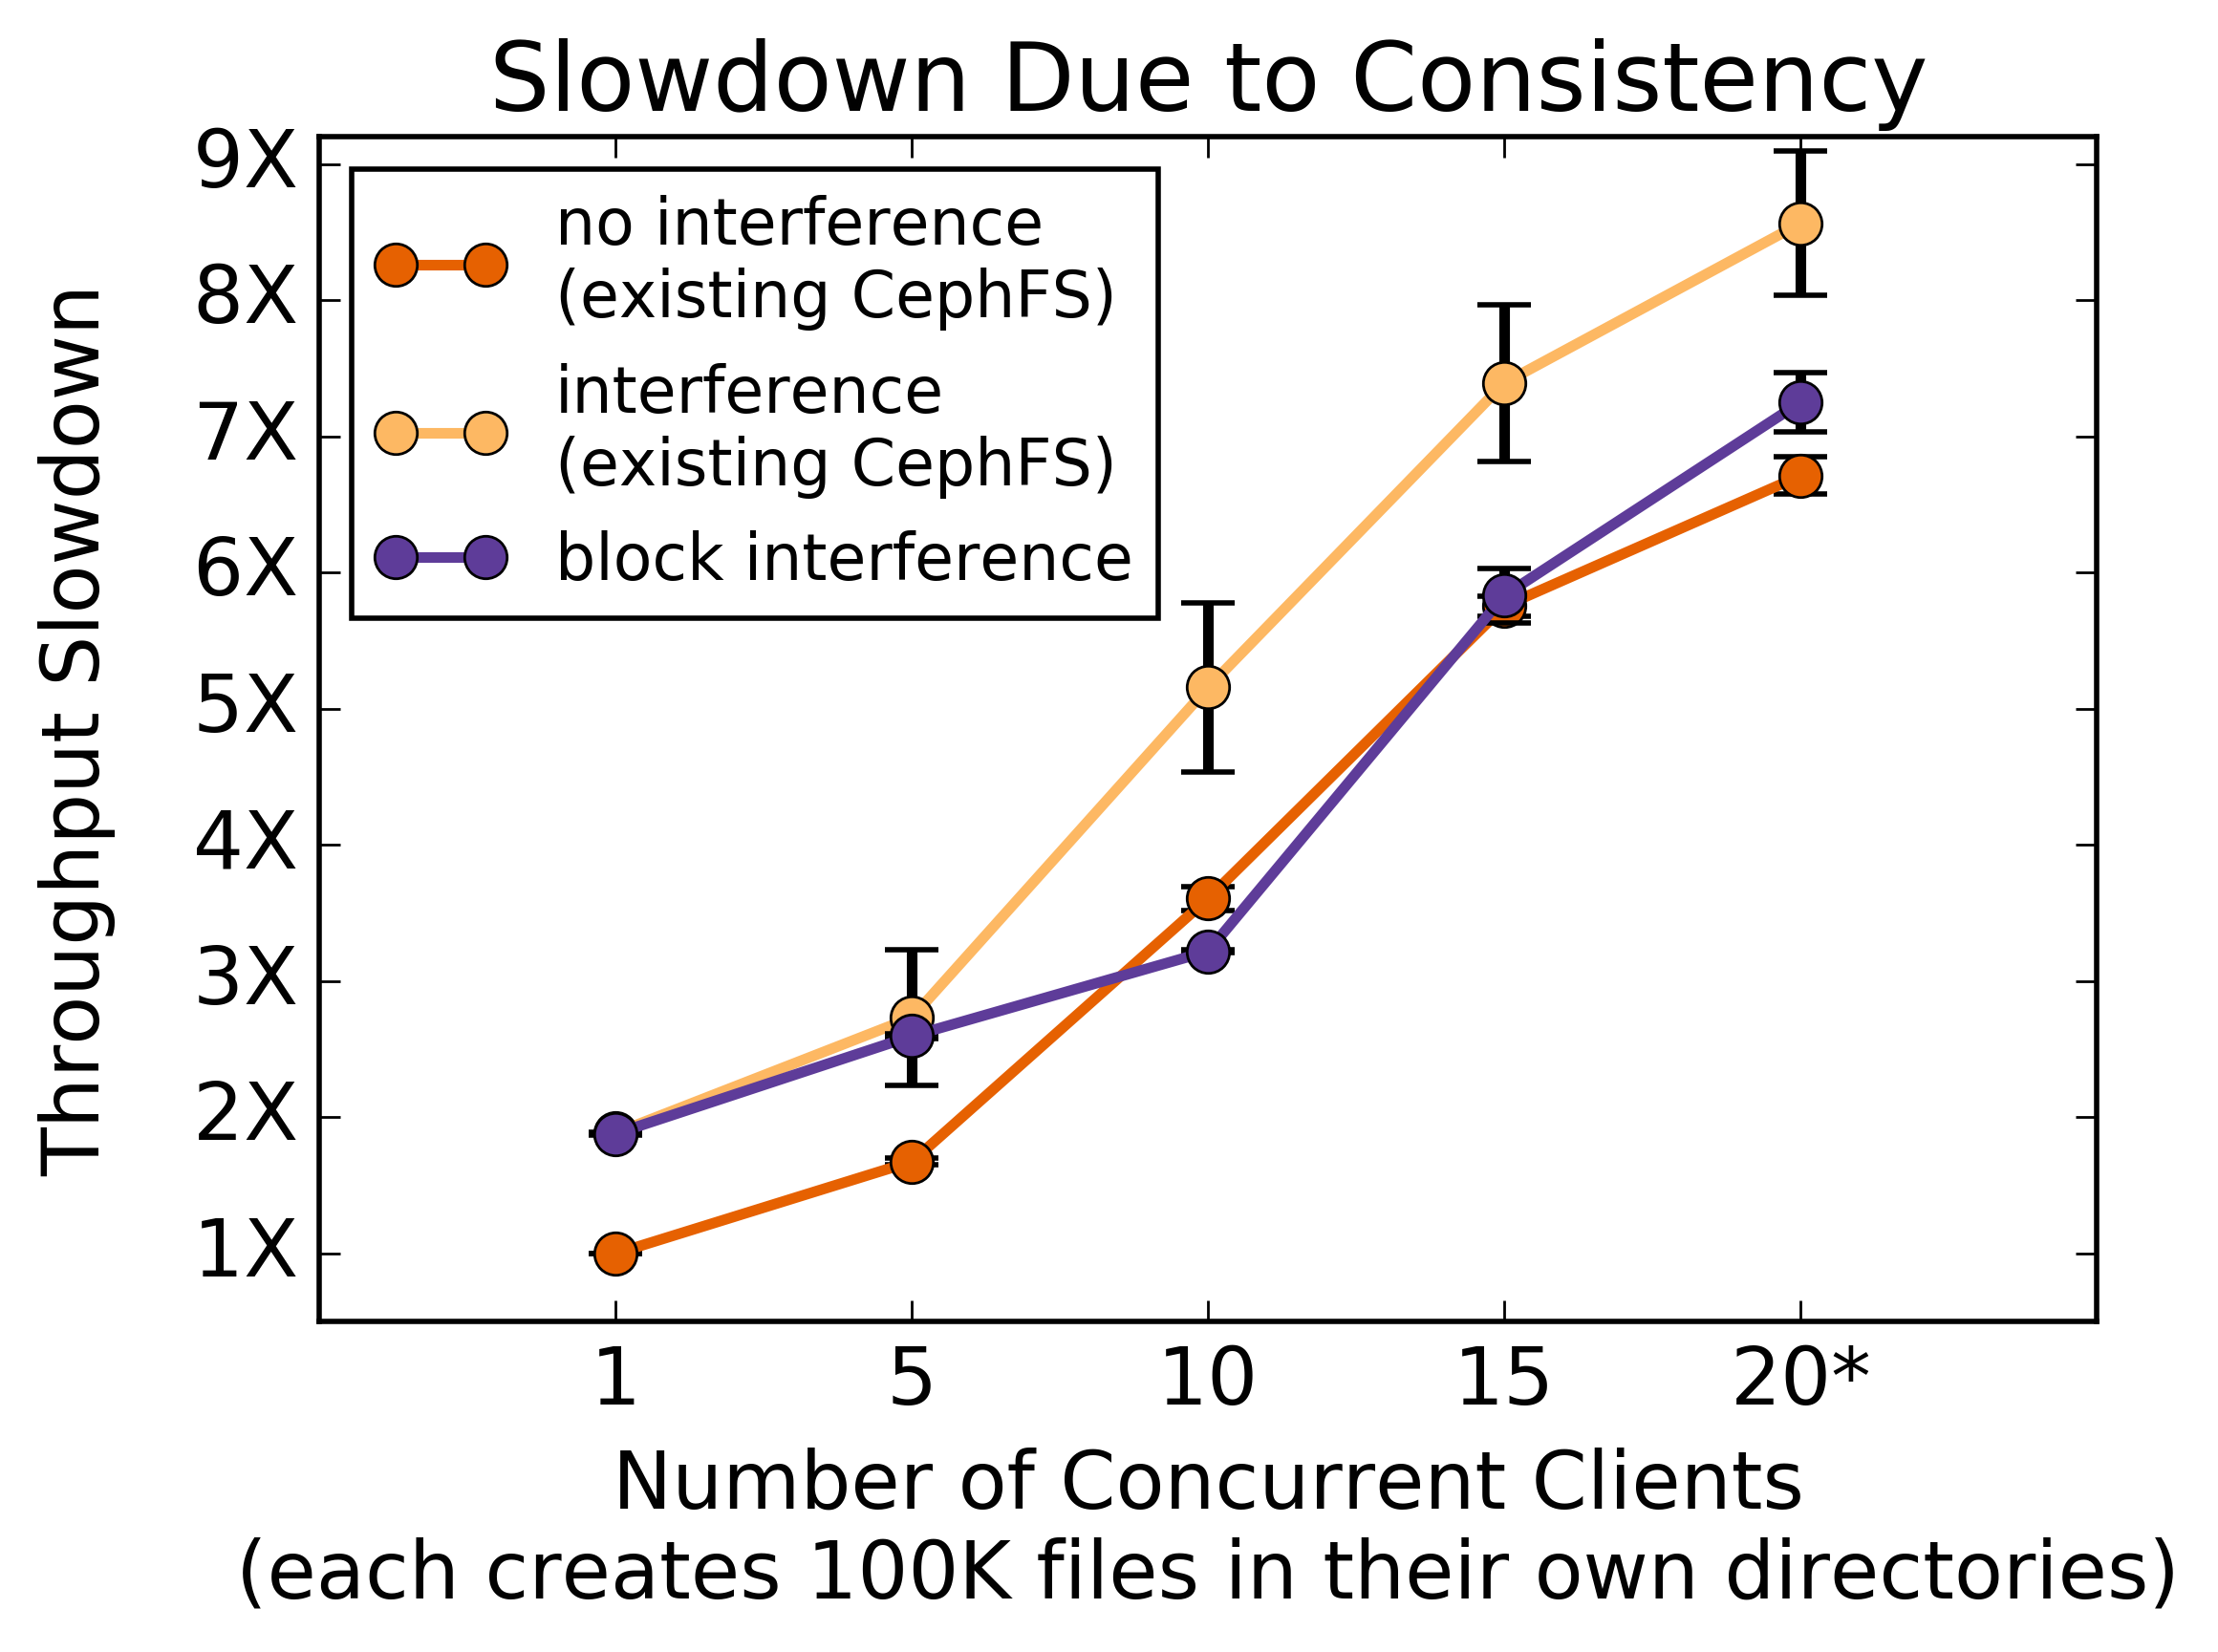
\includegraphics[width=0.5\linewidth]{./chapters/cudele/figures/block-allow.png}
  \caption{
  [\href{https://github.com/michaelsevilla/cudele-popper/blob/master/experiments/cudele-blockapi/visualize/viz.ipynb}{source}]
  The block/allow interference API isolates directories from interfering
  clients.}
  \label{fig:block-allow}
\end{figure}

\begin{figure}
  \centering
  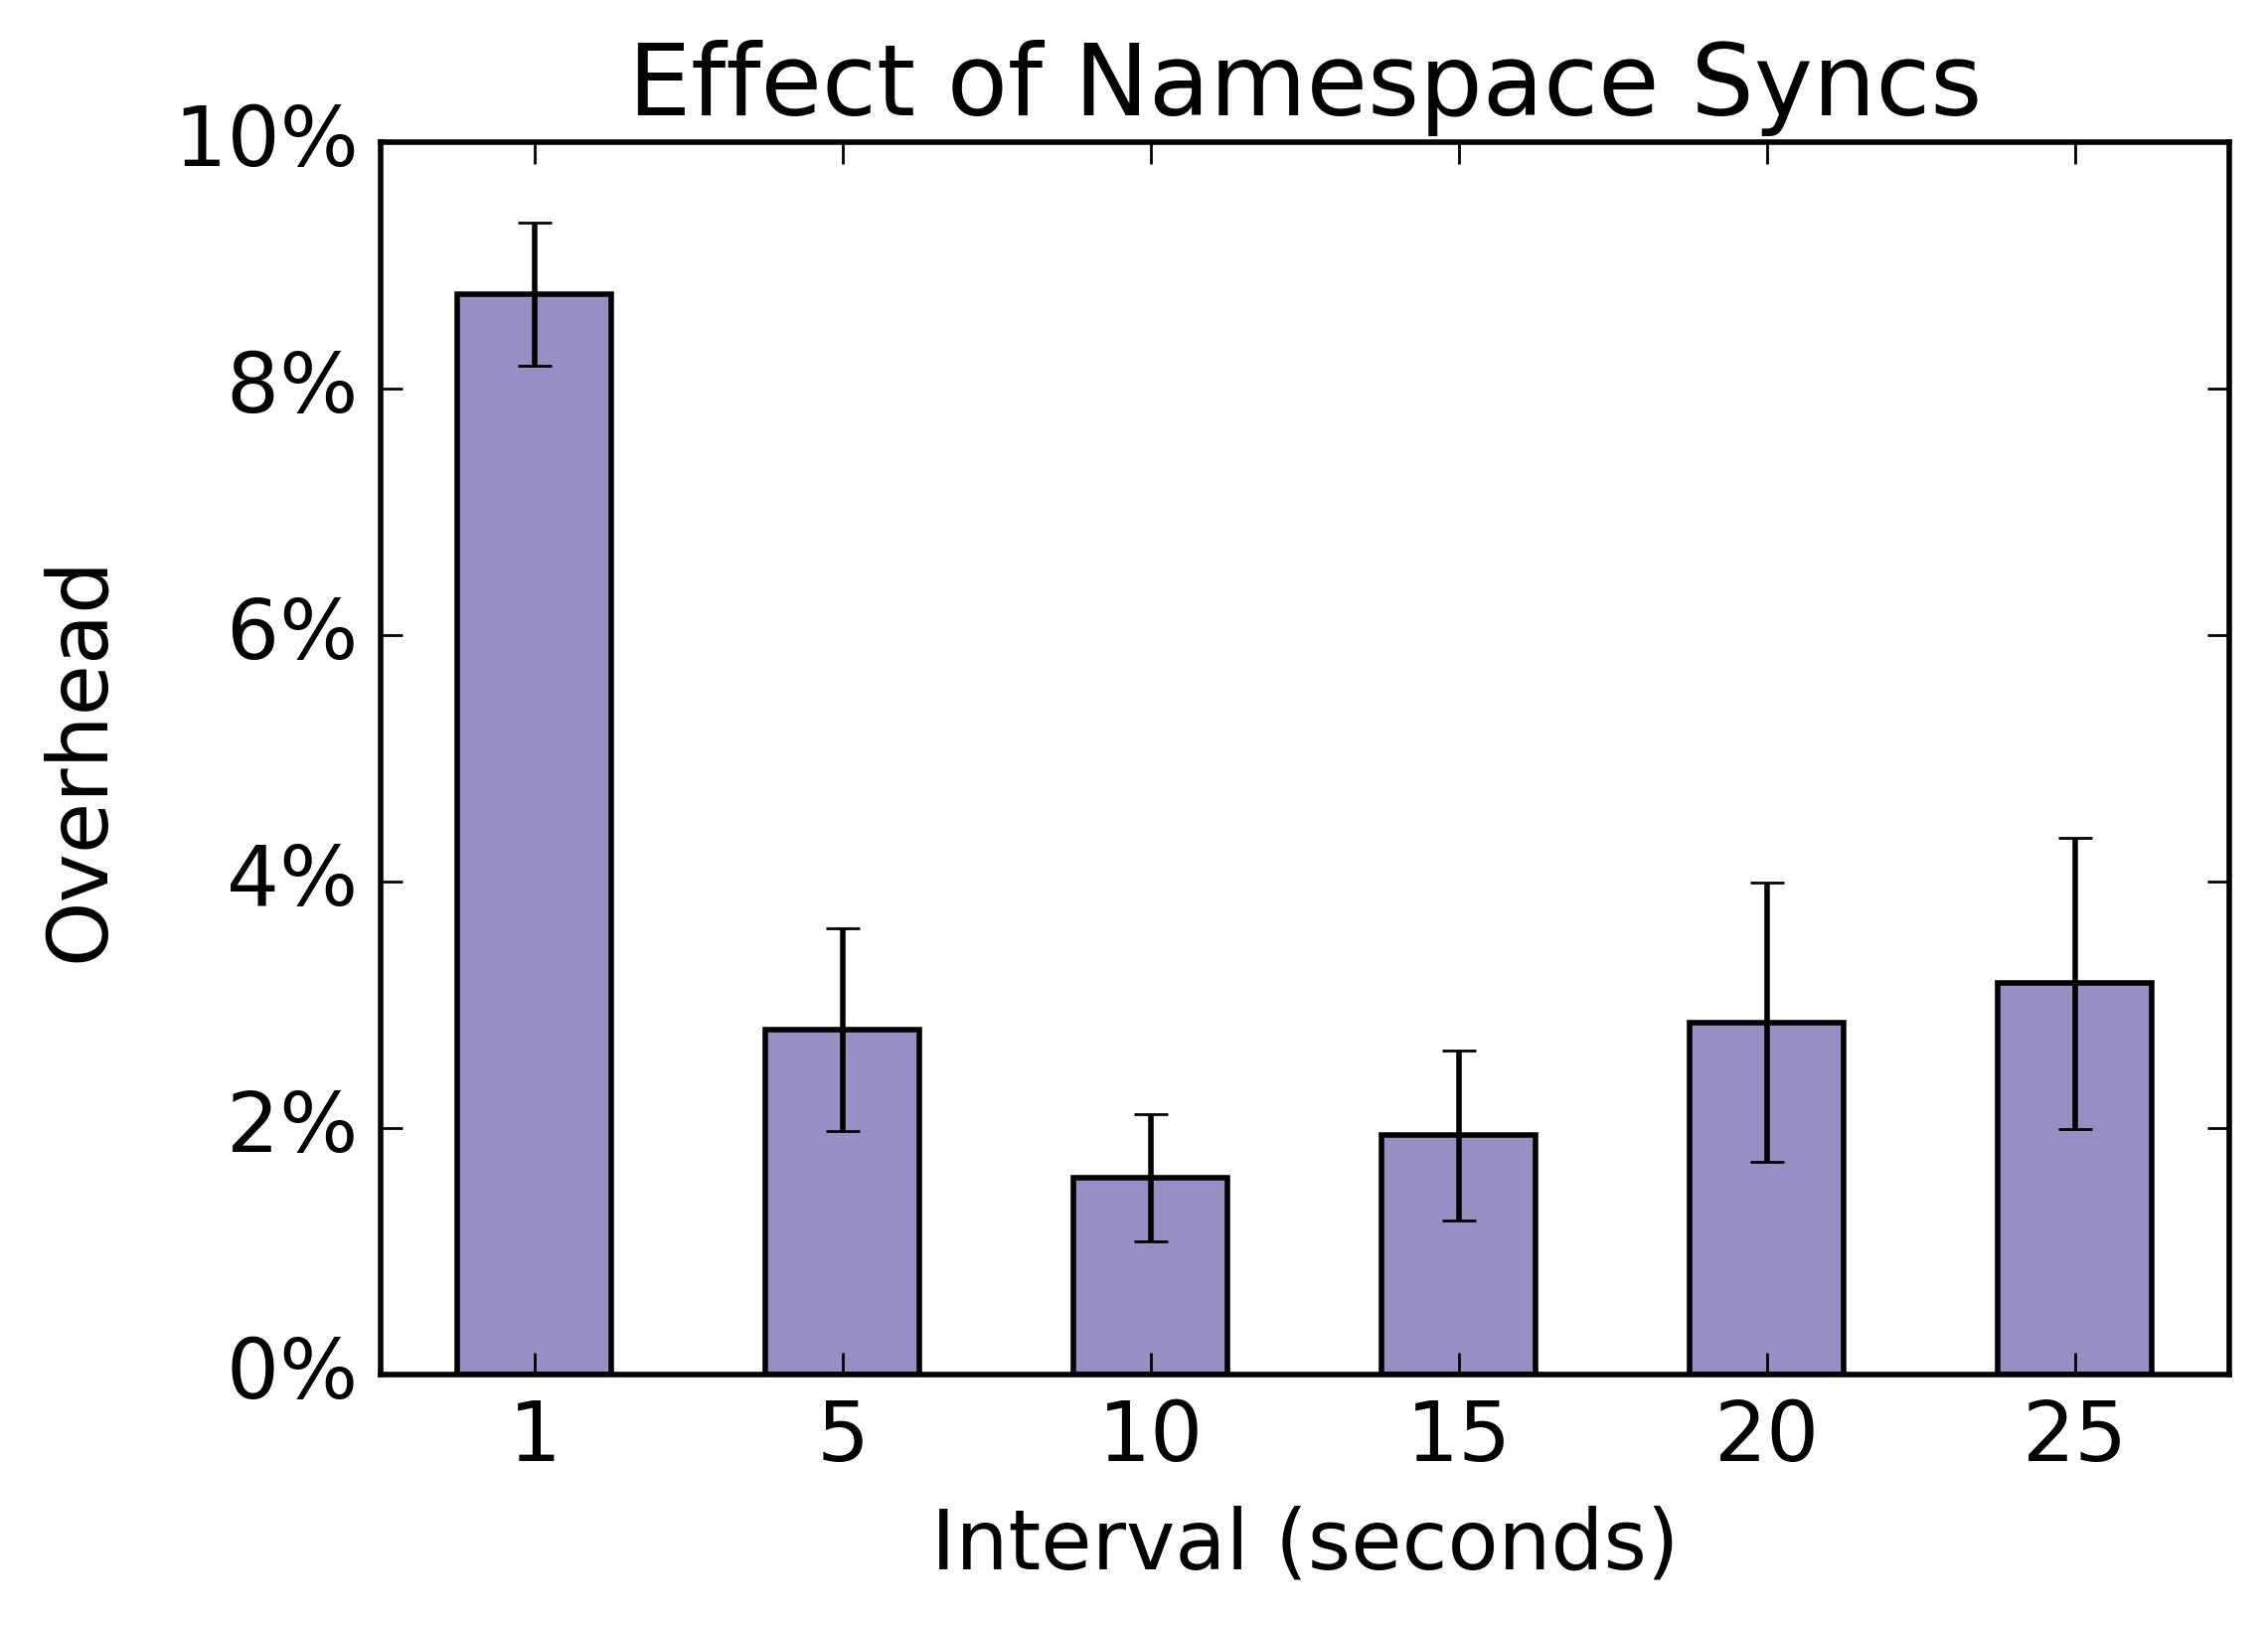
\includegraphics[width=0.5\linewidth]{./chapters/cudele/figures/slowdown-sync.png}
  \caption{
  [\href{https://github.com/michaelsevilla/cudele-popper/blob/master/experiments/cudele-partialreads/visualize/viz.ipynb}{source}]
  Syncing to the global namespace. The bars show the slowdown of a single
  client syncing updates to the global namespace. The inflection point is the
  trade-off of frequent updates vs. larger journal files.}
  \label{fig:slowdown-sync}
\end{figure}

\newcomment{{\it Composing Mechanisms}: The graph on the right of
Figure~\ref{fig:composable-mechanisms} shows how applications can compose
mechanisms together to get the consistency/durability guarantees they need in a
global namespace.  We label the \(x\)-axis with systems that employ these
semantics, as described in Figure~\ref{fig:subtree-policies}.  We make no
guarantees during execution of the mechanisms or when transitioning semantics
-- the semantics are guaranteed {\it once the mechanism completes}.  So if
servers fail during a mechanism, metadata or data may be lost. This graph shows
how we can build application-specific subtrees by composing mechanisms and the performance of
coupling well-established techniques to specific applications over the same file system.}

%results in a more
%scalable global namespace.}

\subsection{Use Cases}

\newcomment{Next we present three uses cases: creates in the same directory,
interfering clients, and read while writing.  The synthetic benchmarks model
scenarios where these workloads co-exist in a global namespace and we provide
insight into how the workload benefits from Cudele.}

\subsubsection{Creates in the Same Directory}
\label{sec:use-case-1}

\oldcomment{Next we show how we can build application-specific subtrees by
composing mechanisms and that this approach of coupling well-established
techniques to specific applications results in a more a scalable global
namespace.} We start with clients creating files in private directories because
this workload is heavily studied in HPC~\cite{weil:sc2004-dyn-metadata,
ren:sc2014-indexfs, patil:fast2011-giga, zheng:pdsw2014-batchfs,
sevilla:sc15-mantle}, mostly due to checkpoint-restart~\cite{bent_plfs_2009}.
For more use cases from other domains like the cloud, see
Section~\S\ref{sec:temporal-locality-during-flash-crowds}.

\newcomment{\textbf{Cudele setup}: accommodate these workloads in the global
namespace by configuring three subtrees with the following semantics: one with
strong consistency and global durability (RPCs), one with invisible consistency
and local durability (decoupled: create), and one with weak consistency and
local durability (decoupled: create + merge).}

%\begin{figure}[tb]
%\centering
%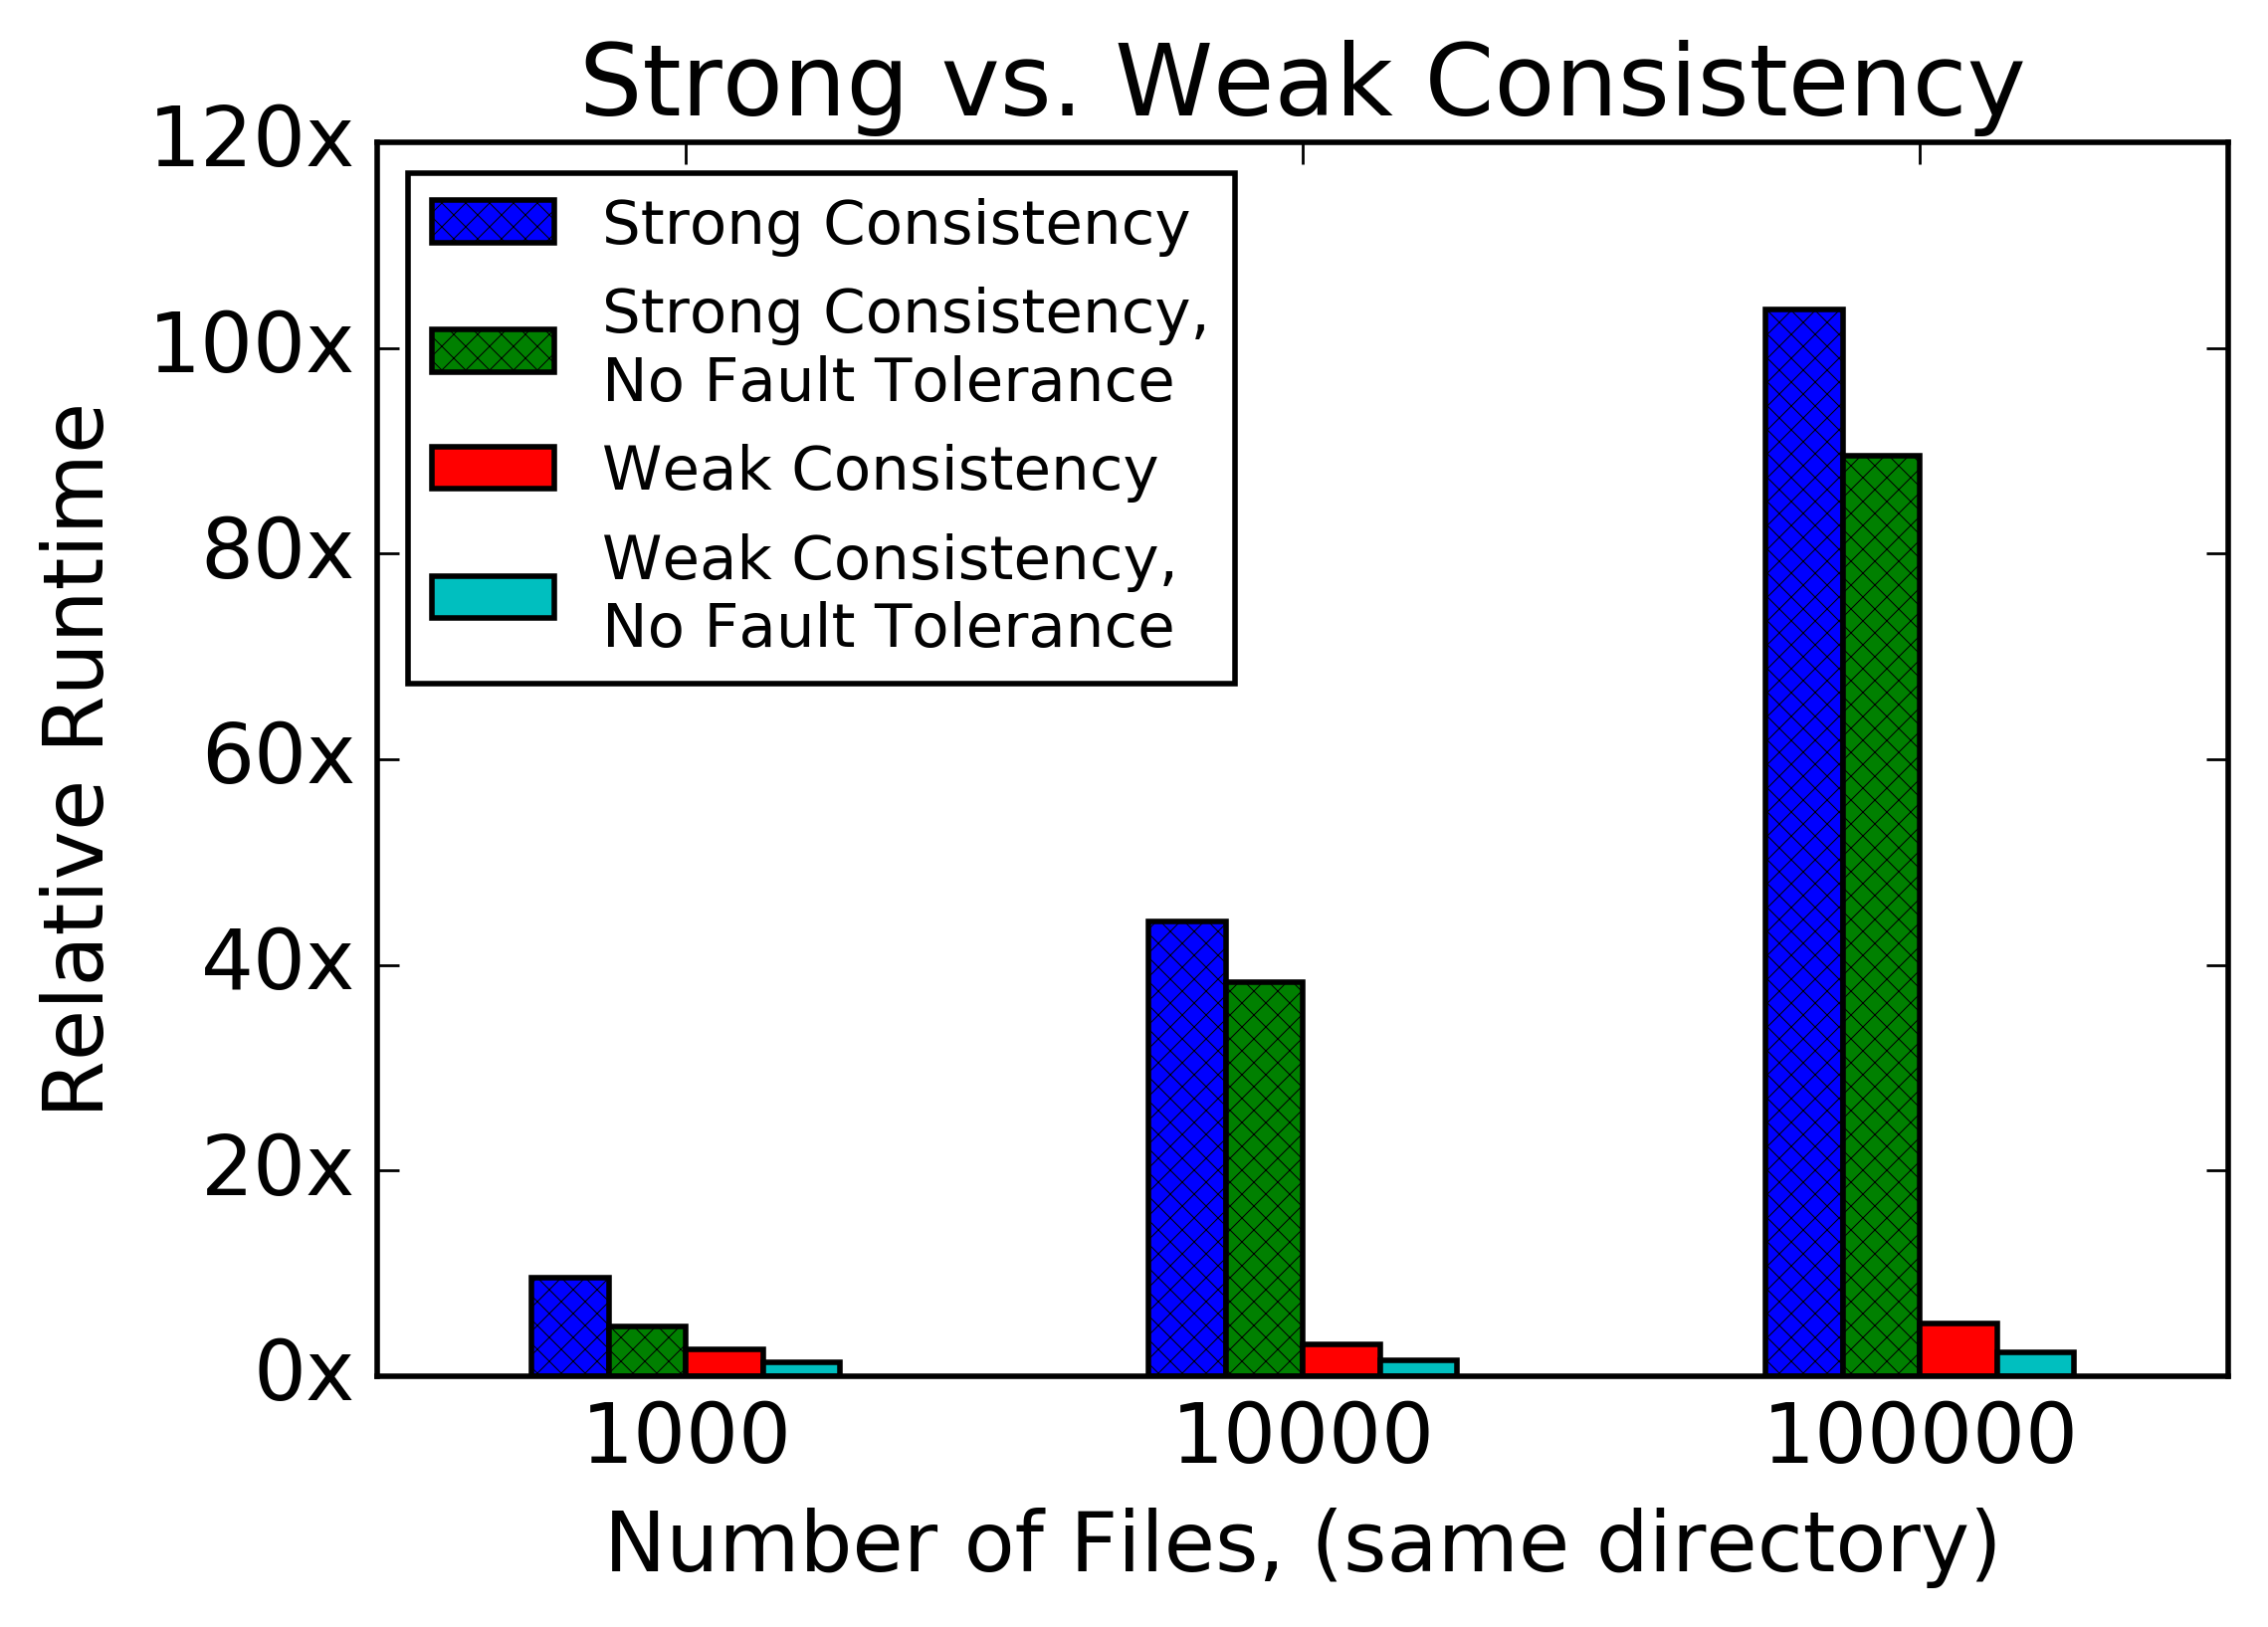
\includegraphics[width=1.0\linewidth]{./chapters/cudele/figures/slowdown-strong-v-weak.png}
%\caption{ [\href{https://...}{source}] Use Case 1: the RPC per metadata update
%(strong consistency) has a large overhead compared to decoupled namespaces
%(weak consistency.)\label{fig:slowdown-strong-weak}}
%\end{figure}

\oldcomment{The graph on the right of Figure~\ref{fig:composable-mechanisms}
shows how applications can compose mechanisms together to get the
consistency/durability guarantees they need in a global namespace.  We label
the \(x\)-axis with systems that employ these semantics, as described in
Figure~\ref{fig:subtree-policies}.  Again, the runtime is normalized to
creating files in the client's in-memory journal.  We make no guarantees during
execution of the mechanisms or when transitioning semantics -- the semantics
are guaranteed {\it once the mechanism completes}. So if servers fail during a
mechanism, metadata or data may be lost.}

\oldcomment{\textbf{Takeaway}: we confirm the performance benefits of other
well-established research systems but, more importantly, we show that the
Cudele mechanisms we propose are useful for building and evaluating different
consistency/durability semantics.\\}

\oldcomment{To show the contention at the metadata server, }In
Figure~\ref{fig:mergescale} we scale the number of clients \newcomment{each
doing 100K file creates in their own directories.  Results are normalized to 1
client that creates 100K files using RPCs (about 549 creates/sec). As opposed
to earlier graphs in Section~\S\ref{sec:posix-overheads} that plotted the
throughput of the slowest client, Figure~\ref{fig:mergescale} plots the
throughput of the total job ({\it i.e.} from the perspective of the metadata
server). Plotting this way is easier to understand because of how we normalize
but the speedups over the RPC approach are the same, whether we look at the
slowest client or not.}

\newcomment{When the metadata server is operating at peak efficiency at
20 clients, the performance of the ``RPCs" and ``decoupled: merge + create"
subtrees is bottlenecked by the metadata server processing power, so the curves
flatten out at a slowdown of \(4.5\times\) and \(15\times\), respectively.  On
the other hand, the ``decoupled: create" subtree performance scales linearly
with the number of concurrent clients because clients operate in parallel and
write updates locally. At 20 clients, we observe a \(91.7\times\) speedup for
``decoupled: create" over RPCs.}\oldcomment{ for the RPC per operation strategy
and the decoupled namespace strategy.  For RPCs, scaling the number of clients
increases the load on the metadata server and for decoupled we increase the
number of concurrent clients operating in parallel.  Related work has pointed
to on-disk metadata format as the primary factor for improved scalability; but
our results show that the weakened consistency and durability enables the
scalability improvements. The on-disk metadata formats in this experiment are
the same for all schemes.}

\newcomment{ ``Decoupled: merge + create" outperforms ``RPCs" by \(3.37\times\)
because ``decoupled: merge + create" uses a relaxed form of consistency and
leverages bulk updates just like DeltaFS~\cite{zheng:pdsw2015-deltafs}.
Decoupled namespaces (1)} place no restrictions on the validity of metadata
inserted into the journal ({\it e.g.}, never checking for the existence of
files before creating files), \newcomment{(2)} avoid touching poorly scaling
data structures\newcomment{, and (3) allow clients to batch events into bulk
updates}. \oldcomment{We can scale linearly if we weaken our consistency by
never checking for the existence of files before creating files ({\it i.e.}
only append \texttt{open()} requests to the journal).  When the updates are
merged by the metadata server into the in-memory metadata store they never scan
growing data structures.}  Had we implemented the \oldcomment{Append Client
Journal mechanism}\newcomment{client to send updates one at a time and} to
include \texttt{lookup()} commands before \texttt{open()} requests, we would
have seen \newcomment{performance closer to the ``RPC" subtree}\oldcomment{the
poor scaling that we see with the RPCs mechanism}. \newcomment{The ``decoupled:
merge + create" curve is also pessimistic because it models a scenario in which
all client journals arrive at the same time.} So for the 20 clients data point,
we are measuring the operations per second for 20 client journals that land on
the metadata server at the same time. \newcomment{Had we added infrastructure
to overlay journal arrivals or time client sync intervals, we could have
scaled more closely to ``decoupled: create".}\oldcomment{The ``create + merge"
bar adds the time it takes for clients to generate the journal of events in
parallel. ALSO DISCUSS 3.7X!!}

%Merge requests are serialized at the metadata server; merging concurrently is
%an optimization for future work. The current implementation has race conditions
%because the metadata server recovery code was not designed to run in parallel
%({\it i.e.} the metadata server never recovers with multiple threads). As a
%result, the metadata server versions inodes and directory entries to ensure
%that the recovered metadata is consistent.

\oldcomment{This workload scales further with decoupled namespaces because the metadata
server is not overwhelmed with RPC requests. Compared to
Figure~\ref{fig:overhead-c} we can scale to 40 clients which is more than
double the capacity of a single metadata server using the RPC strategy to
maintain strong consistency Note that for the 20 clients
bar in Figure~\ref{fig:mergescale}, we plot the throughput for using 18 clients
(the maximum number of clients supported by RPCs). }

\oldcomment{\textbf{Takeaway}: the ability to couple well-established techniques to
specific applications allows the global namespace to scale further and perform
better. In our case, RPCs overwhelm the system but decoupling/shipping a
journal of updates improves scalability by 2\(\times\).}

%\section{notes}
%Linking clients into our custom libcephfs
%
%Use namespace's recursive data structure to put policies on subtrees
%- consistency: weak vs. strong, global vs. local
%  - e.g., BatchFS/DeltaFS: weak, local
%  - e.g., POSIX IO: strong, global
%  - e.g., PLFS: no consistency
%- durability: global vs. local
%  - e.g., CephFS: global
%  - e.g., BatchFS/DeltaFS: local
%
%Experimental Setup
%- Ceph: 9 OSDs, 1 metadata server, 2 kernel client
%- Workload limitations: blah
%
%Workload: creates
%
%Baseline: 200K creates in the same directory
%- throughput: degrades at 950s
%- CPU utilization: more at 950s
%- inode cache: eviction dominate
%- inodes +- to cache: eviction dominate
%- per-disk throughput: RADOS not bottleneck
%
%Experiment 1: Interference
%
%\subsection{Baseline}
%Experiment 0: creates in the same directory
%- setup: why we use caching, we use the kernel client, how we circumvent max fragment size
%
%Experiment 0: creates with a stat
%- Hypothesis: metadata read pauses creates and requires a snapshot in time
%  - what is more of an overhead: pausing creates and getting a consistent view OR sucking up resources as it reads from RADOS?
%- can we delay snapshot?
%
%Experiment 1: creates with a readdir
%- Hypothesis: shows the cost of synchronization because on a write, the first client drops his caps
%- client0: create 100k, client1: stat at 2 mins
%
%Experiment 2: scale the number of files
%- See if the open/close spike occurs 
%- Try to see why open/close spike is allowed to happen
%- Try to disable all caching -- metadata writes don't ever re-use the inode -- we never ask for it again!
%- client0: create 100k, client1: touch at 2 mins
%
%Experiment 3: see how fast the cache satisfies a read
%- client0: create 100k, stat inodes
%- client0: create 100k, client1: stat inodes
%
%lient 0: creates, client 1 create(s)

\subsubsection{Interfering Clients}

Next we show how Cudele can be programmed to block interfering
clients\oldcomment{ using the same problematic workload from
Figure~\ref{fig:overhead-b}. In this workload, c}\newcomment{, which lets
applications control isolation to get better and more reliable performance.}
Clients create 100K files in their own directories while another client
interferes by creating \oldcomment{more}\newcomment{1000} files in each
directory. \oldcomment{This}\newcomment{The workload} introduces false sharing
and the metadata server revokes capabilities on directories touched by the
interfering client. More examples can be found in
Section~\S\ref{sec:spatial-locality-within-directories}.

\newcomment{\textbf{Cudele setup}: enable global durability with Stream and
strong consistency with RPCs to mirror the setup from the problem presented in
Figure~\ref{fig:overhead-b}. We configure one subtree with an interfere policy
of ``allow" and another subtree with ``block" so \texttt{-EBUSY} is
returned to interfering clients.  The former is the default behavior in file
systems and the latter isolates performance from interfering clients.}

\oldcomment{We only scale to 15 clients because the performance variability of
a nearly overloaded metadata server, in our case 18 clients, is too high.}
Figure~\ref{fig:block-allow} plots the overhead of the slowest
client\oldcomment{and the error bars are the standard deviation of 3 runs.
``Interfere (Fig 3c)" is the result from Figure~\ref{fig:overhead-b};
``Interfere" uses the allow/block API to return \texttt{-EBUSY} to interfering
clients; and ``Isolated" is the baseline performance without an interfering.
Each subtree has RPCs and Stream enabled.  Results are normalized to the
runtime of a single client creating files in a directory.  Note that IndexFS
has a similar behavior to ``interfere" with leases, except clients block.
}\newcomment{, normalized to 1 client that creates 100K files in isolation
(about 513 creates/sec). ``Interference" and ``no interference" is the
performance with and without an interfering client touching files in every
directory, respectively. The goal is to explicitly isolate clients so that
performance is similar to the ``no interference" curve, which has lower
slowdowns (on average, \(1.42\times\) per client compared to \(1.67\times\) per
client for ``interference") and less variability (on average, a standard deviation
of 0.06 compared to 0.44 for ``interference").  ``Block interference" uses the
Cudele API to block interfering clients and the slowdown (\(1.34\times\) per
client) and variability (0.09) look very similar to ``no interference" for a
larger number of clients. For smaller clusters the overhead to reject requests
is more evident when the metadata server is underloaded so the slowdowns are
similar to ``interference".  We conclude that administrators can block interfering clients to get the same
performance as isolated scenarios but there is a non-negligible overhead for
rejecting requests when the metadata server is not operating at peak
efficiency.}

\oldcomment{We draw three conclusions: (1) clients that use the API to block
interfering clients  get the same performance as isolated clients, (2) there is
a negligible effect on performance for the extra work the metadata server does
to return \texttt{-EBUSY}, and (3) merging updates from the decoupled client
has a negligible effect on performance.  \textbf{Takeaway}: the API lets users
isolate directories when applications need better and more reliable
performance. Blocking updates is an effective way of controlling consistency.}

\subsubsection{Read while Writing}

The final use case shows how the API gives
\oldcomment{users}\newcomment{administrators} fine-grained control of the
consistency semantics \newcomment{to support current practices and scientific
workflows in HPC}. More details for this use case can be found in
Section~\S\ref{sec:listing-directories}.

% Does this implementation need to be described in the implementation?
\newcomment{\textbf{Cudele setup}: in this scenario, Cudele end-users will not see
the progress of decoupled namespaces since their updates are not globally
visible.  To provide the performance of decoupled namespaces and to help end-users
judge the progress of their jobs, Cudele clients have a ``namespace sync" that
sends batches of updates back to the global namespace at regular intervals.
We configure a subtree as a decoupled namespace with invisible consistency, local
durability, and partial updates enabled.}

Figure~\ref{fig:slowdown-sync} shows the performance degradation of a single
client writing \newcomment{1 million} updates to the decoupled namespace and
pausing to send updates to the metadata server. \oldcomment{The error bars are
the standard deviations of 3 runs.} We scale the namespace sync interval to
show the trade-off of frequently pausing or writing large logs of updates.  We
use an idle core to log the updates and to do the network transfer. The client
only pauses to fork off a background process, which is expensive as the address
space needs to be copied. The alternative is to pause the client completely and
write the update to disk but since this implementation is limited by the speed
of the disk, we choose the memory-to-memory copy of the fork approach.

As expected, syncing namespace updates too frequently has the highest overhead
(up to 9\% overhead if done every second). The optimal sync interval for
performance is 10 seconds, which only incurs 2\% overhead, because larger
intervals must write more updates to disk and network. For the 25 second
interval, the client only pauses 3-4 times but each sync writes about 278
thousand updates at once, which is a journal of size 678MB.

\oldcomment{\textbf{Takeaway}: Syncing namespace updates has up to a 9\%
overhead and can be tuned depending on the users preference but, more
importantly, the API gives users fine-grain control of their
consistency/durability to support current practices or experimental workflows.}

%\subsection{Use Case 4: Reading Large Directories} 
%
%% CITEME
%The final use case is reading large directories. At job completion, scientists
%might use \texttt{ls} again to see the results. This causes great strain on the
%file system as paths need to traversed and the entire directory, with all its
%entries, must be transferred back to the client. Here we show how decoupling a
%large namespace and materializing the view in memory on the client is faster
%than doing RPCs for walks of the file system namespace.
%
%FigureX shows how fast a client can materialize decoupled namespaces in memory.
%This takes the on-disk file system metadata format and parses them into events
%that can be manipulated and appended to. Again, we scale the number of up

%\subsection{Discussion and Future Work}
%
%\newcomment{We have shown that our API and framework is an effective
%abstraction for letting \oldcomment{users}\newcomment{administrators} custom
%fit subtrees to applications.  

%Second is the opportunity for adding hardware in strategic places to speed up
%the mechanisms that the application needs. In Figure~\ref{fig:mergescale} the
%performance of merging updates at the metadata server is limited by the speed
%of the disk. So applications that rely on merging many updates should consider
%equipping the metadata server with SSDs or more memory. 
%

